\chapter{Introduction and Motivation}
\label{thesis:introduction}



Internet of Things (IoT) is transforming the world of things into an autonomous world. It has a high impact in many industries such as manufacturing, transportation, automotive, consumer goods, and even healthcare will never be the same
once IoT is applied. Thanks to the advances of the underlying technologies, IoT devices are being equipped with more powerful processors and are able to effectively distribute the processing load to other cores. This offers the opportunity of to run more complex tasks in the IoT devices. In our study we are going to use ESP EYE (reference) which is equipped wit camera and microphone which comes with plenty of storage with an 8 Mbyte PSRAM and a 4 Mbyte flash. 
However IoT comes with a number of challenges or gaps  that still need to be improved such as: security issues, centralization and the vulnerability to attacks. 
On the other hand blockchains as a decentralized network is able to hold to records and transactions in blocks secured by cryptography. We can see that the advantages of blockchain converge with the disadvantages of IoT which can eventually transform how information is processes and stored. On the other hand Artificial Intelligence (AI) has a significant role as an accurate analysis of data in real time. However with the design and development of an efficient data analysis tool  using AI comes with challenges : centralized architecture, security issues and the decisions made from AI are not transparent and recorded. Therefore integrating the blockchain with AI has the ability to produce a robust technology to resolve the several AI issues. AI as a black box box lacks transparency, therefore with the transparency of blockchain with sharing the data in many nodes in a subsequent order provides a clear way for tracking back the data to the AI decision process.   

Therefore the convergence of the three domains will bring a successful synergy that will transform how data is being processed, analyzed and stored. In this study we aim to explore the three mentioned emerging paradigms that will influence the future. Therefore the main goal of this research is the design and development of a Blockchain-enabled Intelligent IoT Architecture with Artificial Intelligence that will provide an efficient implementation of a use case while incorporating the three domains with the most state of the art technologies and applications. 
There are a number of attempts that shed light on the benefits of converging IoT, blockchain and AI (reference) but most of them are either reviews or explorations but far away from a concrete implementation of a use case (ref2). A more close research in the this matter is an attempt (ref) which proposes a BlockIoTIntelligence architecture as they call it that converges the blockchain, AI for IoT whose aim is to achieve the goal of big data analysis, security and centralization issues of IoT applications such smart city, healthcare and smart transportation. With their findings they claim that BlockIoTIntelligence can mitigate the existing challenges and obtain high accuracy with a reasonable latency and security in the decentralized way. 
If narrowing down the scope to blockchain and IoT we see a slightly more research who attempt to close the gaps of IoT by removing the centralized control with the help of blockchain (refmyown).
For example [ref3]attempted to find out the security and privacy in IoT  gaps that could be filled with the help of the blockchain to ensure the reliability and availability of the data. 

Having had a closer look on the research that shed light on the synthesis of the three domains we see a number of proposals and architecture but yet we do not see a real use case where the three technologies can complement each other. 
Therefore the main goal of this project is to design and implement an IoT surveillance system with blockchain and AI to support access control with facial detection and recognition. Therefore the use case we are designing and implementing provides an efficient way of converging blockchain, AI and IoT with the most current state-of-the-art approaches. 
We are entering an age where surveillance is becoming a norm and facial recognition technologies are hunting the streets. The roll out of facial recognition technologies is expected to become more prominent and an important step in improved security. On the other side, major data breaching has become common place and people worry about the type of personal information held by organizations. In the midst of the COVID-19 pandemic, attention have turned to facial recognition technology as a way to combat the spread of the virus.

Before introducing our own architecture an interesting use case that resembles  our architecture is an implementation of a camera based sensor for monitoring room occupancy. 

Hence to combat the many issues we have discussed and found in the above use case we will be using a low powered IoT device named ESP EYE which with the help of AI running on it will detect and recognize the individuals and grant or reject access. In the due time the ESP EYE will capture images of individuals and forwards them to the blockchain where it will be stored. The proposed architecture and implementation paves the way towards a strong architecture that fills the many gaps of the three domains. Therefore the main goal of this project is to design and implement an IoT-based surveillance system with blockchain and AI to support access control with facial detection and recognition. 
The Face detection and recognition is done in the ESP EYE itself with the help of two machine learning algorithms. For the face detection we employee the MTCNN (Multi-task Cascaded Convolutional Neural Networks ). With the help of FRMN ( Human Face Recognition Model) the person will be recognized. 



% ~\cite{morin}.
%~\cite{what_is_lora}.





 
 


\section{Description of Work}
First of all this study provides an introduction to an IoT architecture using the ESP EYE device which runs a Convolutional Neural Networks (CNN) for face detection and recognition. In addition to that the architecture also shows how the ESP EYE is enabled to issue transactions to a blockchain. The main contributions of the thesis is not only the design but also the implementation of a use case with the above mentioned technologies. We have proposed an IoT surveillance system which is based on blockchain that jointly work together for authentication of people allowed to enter a building. By employing a face recognition IoT device named ESP eye we can do the verification and identification of allowed people to enter an institution without any physical interaction required by the end-user. The are three main milestones of this research. First, we will give a high level approach of the architecture while specifying the technologies and algorithms to be used and the reason behind choosing such technologies. Furthermore, we will introduce the technologies and their architecture and will evaluate against other similar technologies. After that we will evaluate the Convolutional Neural Networks for resource constraints devices which are applied for face detection and recognition. In addition we will also have a closer look at the Hyperledger Fabric to be used in this architecture. Hyperledger Fabric will be evaluated and we will compare and contrast with other blockchain technologies. 
The main section of the thesis will be about the design and implementation details of the Blockchain-enabled Intelligent IoT surveillance system. The ESP EYE will run the Convolutional Neural Networks a Deep Learning algorithm for face detection and recognition. Besides, we will prove how the ESP EYE is able to issue transactions to Hyperledger Fabric. We are going to use Hyperledger Fabric to accommodate the need of IoT devices where in our case it will be sending images of recognized and non recognized individuals in the form of transactions. 



\section{High Level Overview}

We know that AI and Blockchain are the leading innovations we witness today. Being the most disrupting technologies, we often talk about their advantages but yet we do not see a real use case. Hence in this section we will provide a high level description of the proposed surveillance system using facial recognition for access control. The system employees a real time face detection and recognition of authorized individuals to grant access to an institution. This means that access is granted and the door opens automatically for him or her without the need to touch anything. Every time an individual needs access a picture of him or her is taken and is then stored in the blockchain. Access is revoked when an individual is not registered in the system but yet a picture of the individual is taken and stored in the blockchain. Once a stranger is detected continuously a warning is raised to inform the administrators for the issue. Simultaneously, the number of people entering and leaving an institution or a room can be tracked. Tracking the number of people entering or leaving the room can be very beneficial in many situations, such as the number of students taking an exam or their presence in a classroom. The use case diagram can be seen in the Figure~\ref{fig:use_case}. 

\begin{figure}[!htb]
    \centering
    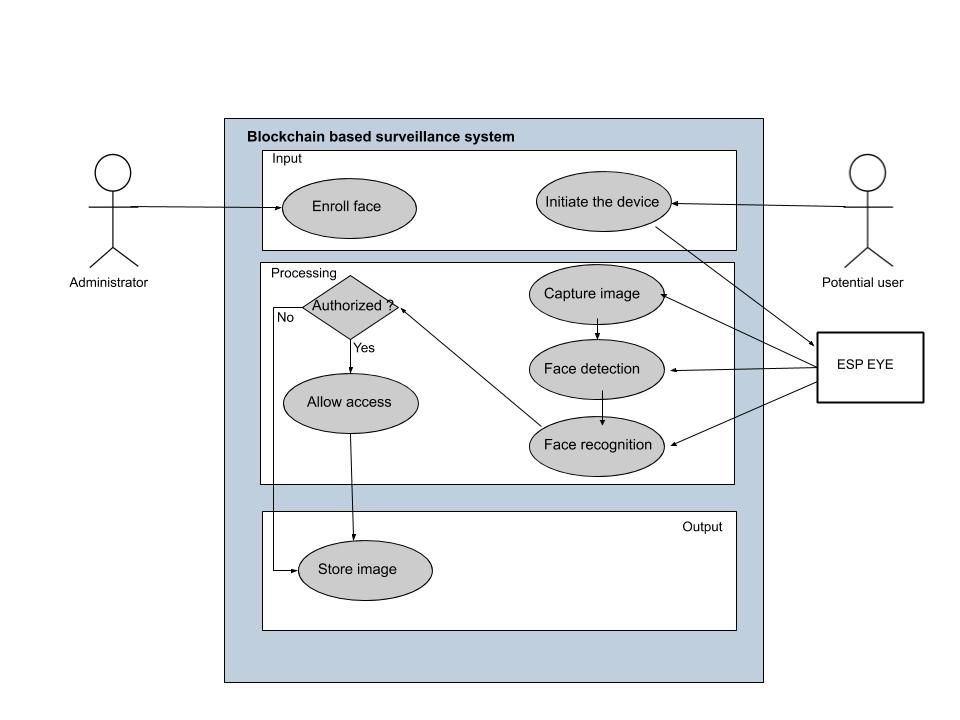
\includegraphics[width=1\textwidth]{figures/use_case.jpg}
    \caption{High Level Overview}
    \label{fig:use_case}
\end{figure}


The assumptions is that the authorized users or individuals are first registered with the system. If an individual is not registered with the system then access is revoked. The process involves an individual approaching an entry point of an institution or a room, where the ESP eye device will detect and recognize the person and grant or reject access. In the due time the ESP WHO platform captures images of individuals and forwards them to the blockchain where it will be stored. Also the cases are considered when a person appears for a continued presence in front of the device. The system shall warn the administrators in such cases. In case of disobedience the system may raise an alarm. 






\section{Thesis Outline}
The rest of the thesis is enumerated in the following order: The second chapter will give a high level approach of the architecture, the hardware used and the design choices that match with the use case which will be compared against other technologies and protocols.

In Chapter ~\ref{chap:lora_and_lorawan} we will introduce and discuss the face detection and recognition algorithms using MTMN which refers to MTCNN (Multi-task Cascaded Convolutional Neural Networks ) and MN (Mobile Nets) for face detection and HFRM (Human Face Recognition Model ) for face recognition. The input for the face detection MTMN is an image captured by the ESP EYE camera and the output is the aligned face which will be as an input for FRMN for face recognition. 

With Hyperledger Fabric we are going add security with the decentralised system by storing all the images of detected individuals. Therefore in order to see the implementation details, its components and the advantages we have allocated Chapter 4 for this. 

In the following chapter, we will dig deeper in the implementation by showing the details of all involved components, the interactions between the components and analyzing the whole architecture. 


In the second-last chapter discusses the future work and improvements of the proposed architecture. Besides  it also lists some limitations that were either coming from the use case or from the technologies. 

Finally, the last chapter encapsulates the whole work by writing the last remarks.

In chapter~\ref{chap:cran_in_cellular}

Chapter~\ref{chap:lora_tools} 


